\begin{figure*}[t]
\centering
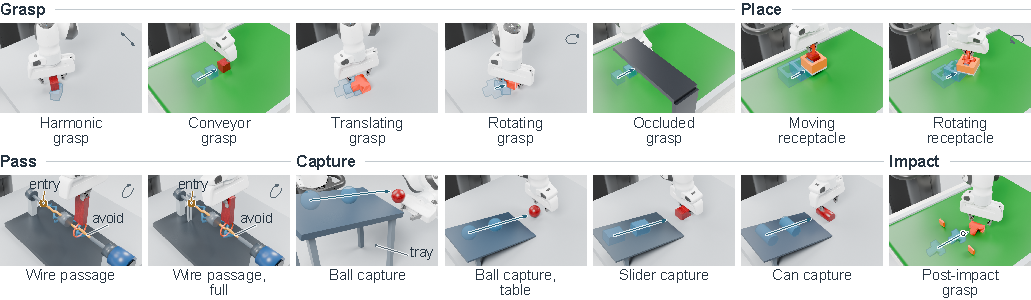
\includegraphics[width=\textwidth]{figures/Fig4/dynamic14.pdf}
\caption{\textbf{\bench.} Fourteen tasks in five families, rendered from recorded
simulator states with a common agent view. Translucent blue poses show selected
history, fading with age; navy traces follow recorded past motion. Gray corner
arrows indicate rotation or oscillation qualitatively. A small ring marks the
target center during recorded impact. Both Pass panels show passage: the wire is
a target at entry and an obstacle along the path; Full additionally requires
acquisition, exit and release. Occluded motion stays hidden. These native-expert
examples illustrate task dynamics, not \ours outcomes; no future prediction is
shown.}
\label{fig:bench_overview}
\end{figure*}
